%% LyX 2.3.7 created this file.  For more info, see http://www.lyx.org/.
%% Do not edit unless you really know what you are doing.
\documentclass[aspectratio=169]{beamer}
\usepackage{lmodern}
\renewcommand{\sfdefault}{lmss}
\renewcommand{\ttdefault}{lmtt}
\usepackage[T1]{fontenc}
\usepackage[utf8]{inputenc}
\setlength{\parindent}{0cm}
\usepackage{amssymb}
\usepackage{graphicx}

\makeatletter
%%%%%%%%%%%%%%%%%%%%%%%%%%%%%% Textclass specific LaTeX commands.
% this default might be overridden by plain title style
\newcommand\makebeamertitle{\frame{\maketitle}}%
% (ERT) argument for the TOC
\AtBeginDocument{%
  \let\origtableofcontents=\tableofcontents
  \def\tableofcontents{\@ifnextchar[{\origtableofcontents}{\gobbletableofcontents}}
  \def\gobbletableofcontents#1{\origtableofcontents}
}

%%%%%%%%%%%%%%%%%%%%%%%%%%%%%% User specified LaTeX commands.
%\usetheme{Warsaw}
%\usetheme{Pittsburgh}
\usetheme{Oxygen}
% or ...

%\setbeamercovered{transparent}
%\setbeamertemplate{headline}{}

\setbeamercovered{dynamic}
\setbeamertemplate{navigation symbols}{}


\definecolor{blue}{RGB}{0,102,255}
\definecolor{Babyblue}{rgb}{0.54, 0.81, 0.94}
\definecolor{mainblue}{RGB}{51, 51, 178}

\usepackage{color, colortbl}
\usepackage{xcolor}
\usepackage[utf8]{inputenc}

\usepackage{movie15}
\usepackage{animate}
\usepackage{graphicx}

\usepackage{array}
\usepackage{booktabs}
\usepackage{amssymb}
\usepackage{svg}
\usepackage{media9}
\usepackage{ulem}
\usepackage{amssymb}
\usepackage{pifont}

\usepackage[edges]{forest} 
\usepackage{tikz}
\usepackage{tikz-qtree}

\usepackage{forest}
\forestset{
  qtree/.style={
    baseline,
    for tree={
      parent anchor=south,
      child anchor=north,
      align=center,
      inner sep=1pt,
    }}}
\usepackage{flexisym}


%\renewcommand\makebeamertitle{{\logo{
\includegraphics[width=4cm]{assets/EscudoUN-2016_styledv2.png}\vspace{0.75cm}}\maketitle}}
\renewcommand\makebeamertitle{{
	\setbeamertemplate{headline}{} 
	\setbeamertemplate{footline}{} 
	\begin{frame}{} 
		\vspace{0cm}     
		\titlepage
	\end{frame}
}}


\newcommand\ungraphic{{
	\vspace{-0.5cm}
	
\includegraphics[width=0.1\textwidth]{assets/EscudoUN.png}\\
	\scriptsize{
		Universidad Nacional de Colombia\\
		Signal Processing and Recognition Group - SPRG\\
		Manizales, Colombia\\
		\today
	}
}}

\makeatother


\begin{document}
\title[Multimodal Data Exchange Systems for Enhanced Interaction and Management]{Multimodal Data Exchange System for\\Enhanced Interaction and Management}
\author{Yeison Nolberto Cardona-Álvarez}
\institute{\textbf{Advisor:} Andrés Marino Álvarez-Meza, Ph.D\\
\textbf{Co-Advisor:} César Germán Castellanos-Domínguez, Ph.D}
\titlegraphic{\ungraphic}
\date{}

\makebeamertitle

%% \AtBeginSection[]{\frame<beamer>{\frametitle{Outline}\tableofcontents[currentsection,currentsubsection]}}

\let\oldcite\cite
\renewcommand*\cite[1]{{\color {gray}\tiny{\oldcite{#1}}}}
\newcommand*\citet[1]{{\color {gray}\fontsize{4}{4}\selectfont{\oldcite{#1}}}}

\begin{frame}{Outline}

\tableofcontents{}
\end{frame}

\section{Motivation}
\begin{frame}{Motivation}

\framesubtitle{Data Exchange: Definition}

Data Exchange refers to the \textbf{efficient and secure} flow of
data between different platforms and procedures \cite{zhang2021fault,thakare2021secure}.

\vfill{}

\begin{figure}
\centering{}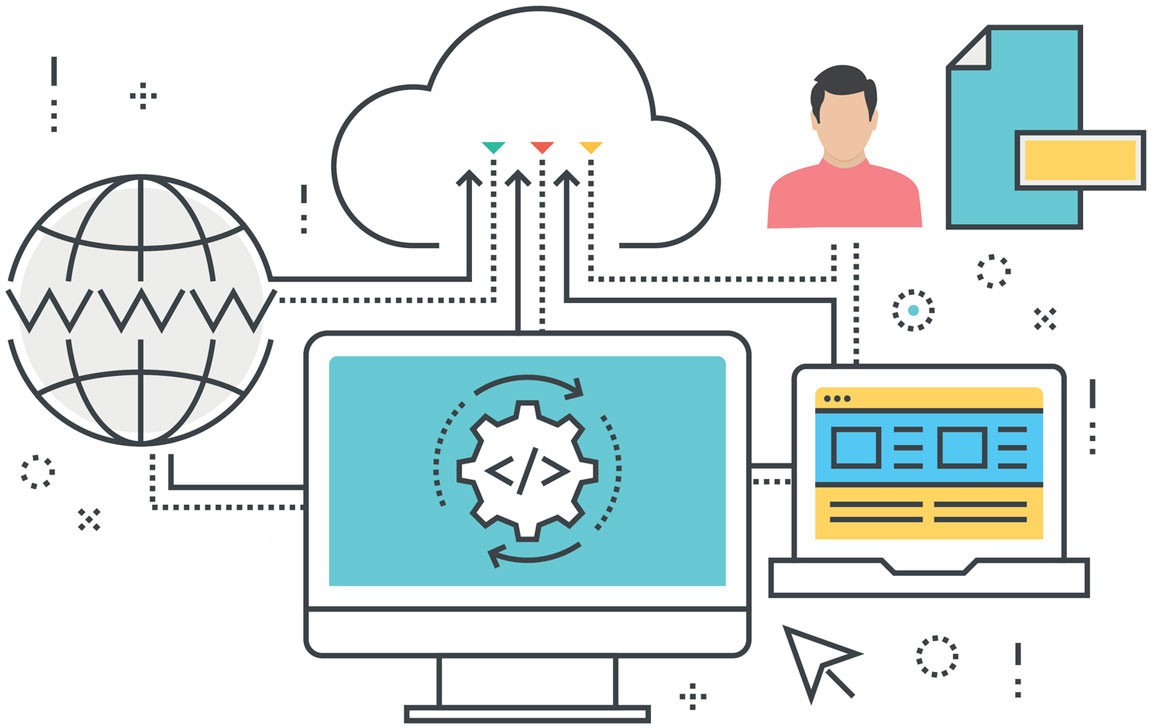
\includegraphics[width=0.3\textwidth]{images/data_exchange_1}
\end{figure}
 

\end{frame}
%
\begin{frame}{Motivation}

\framesubtitle{Data Exchange: Applications and Investments}

It requires strong security and encryption, data quality and dependability,
and industry-specific \textbf{compliance standards} \cite{attiogbe2021advances}.
\begin{columns}[t]

\column[b]{0.66\textwidth}
\begin{itemize}
\item {\scriptsize{}Business intelligence and analytics \cite{kouper2021challenges}. }{\scriptsize\par}
\item {\scriptsize{}Finance and banking \cite{Elsaify2021Data}.}{\scriptsize\par}
\item {\scriptsize{}Government and public services \cite{Ball2020Organizational}.}{\scriptsize\par}
\item {\scriptsize{}Marketing and advertising \cite{mishra2023application}.}{\scriptsize\par}
\item {\scriptsize{}Healthcare \cite{al2022application}.}{\scriptsize\par}
\item {\scriptsize{}Research and academia \cite{qiu2021comprehensive,paltun2021diverse,adiga2022enhancing}.}{\scriptsize\par}
\end{itemize}

\column[b]{0.34\textwidth}

{\scriptsize{}}{\scriptsize\par}

\begin{figure}
\centering{}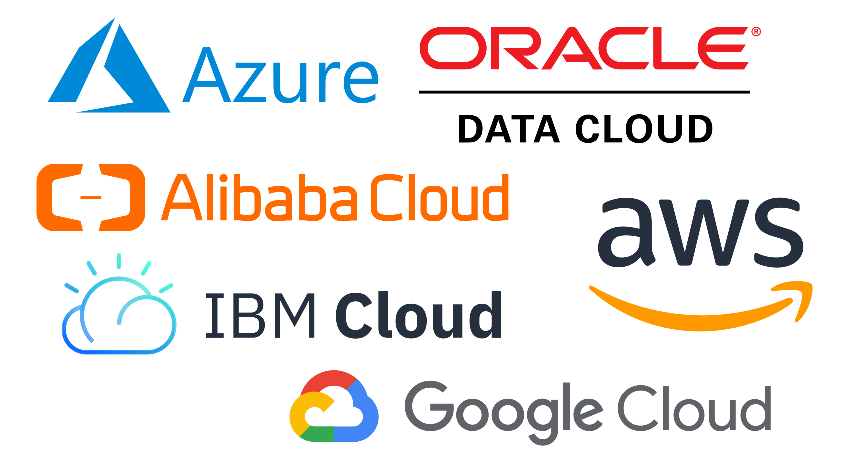
\includegraphics[width=1\columnwidth]{images/datacenters}
\end{figure}

\end{columns}

\end{frame}
%
\begin{frame}{Motivation}

\framesubtitle{The Growth of Data Centers in Colombia}

Latin America's technological revolution plays a crucial role in promoting
\textbf{regional economic growth}, closing the digital gap, creating
a foundation for improved connectivity, innovation, and robust digital
infrastructure \cite{KearneyGlobalServices2023}.
\begin{columns}[t]

\column[b]{0.6\textwidth }
\begin{itemize}
\item {\scriptsize{}Fourth largest data center market in Latin America.
}{\scriptsize\par}
\item {\scriptsize{}Significant investments in infrastructure. }{\scriptsize\par}
\item {\scriptsize{}Attractive for international investments. }{\scriptsize\par}
\item {\scriptsize{}Strategic location advantage. }{\scriptsize\par}
\end{itemize}

\column[b]{0.4\textwidth }

\begin{figure}
\centering{}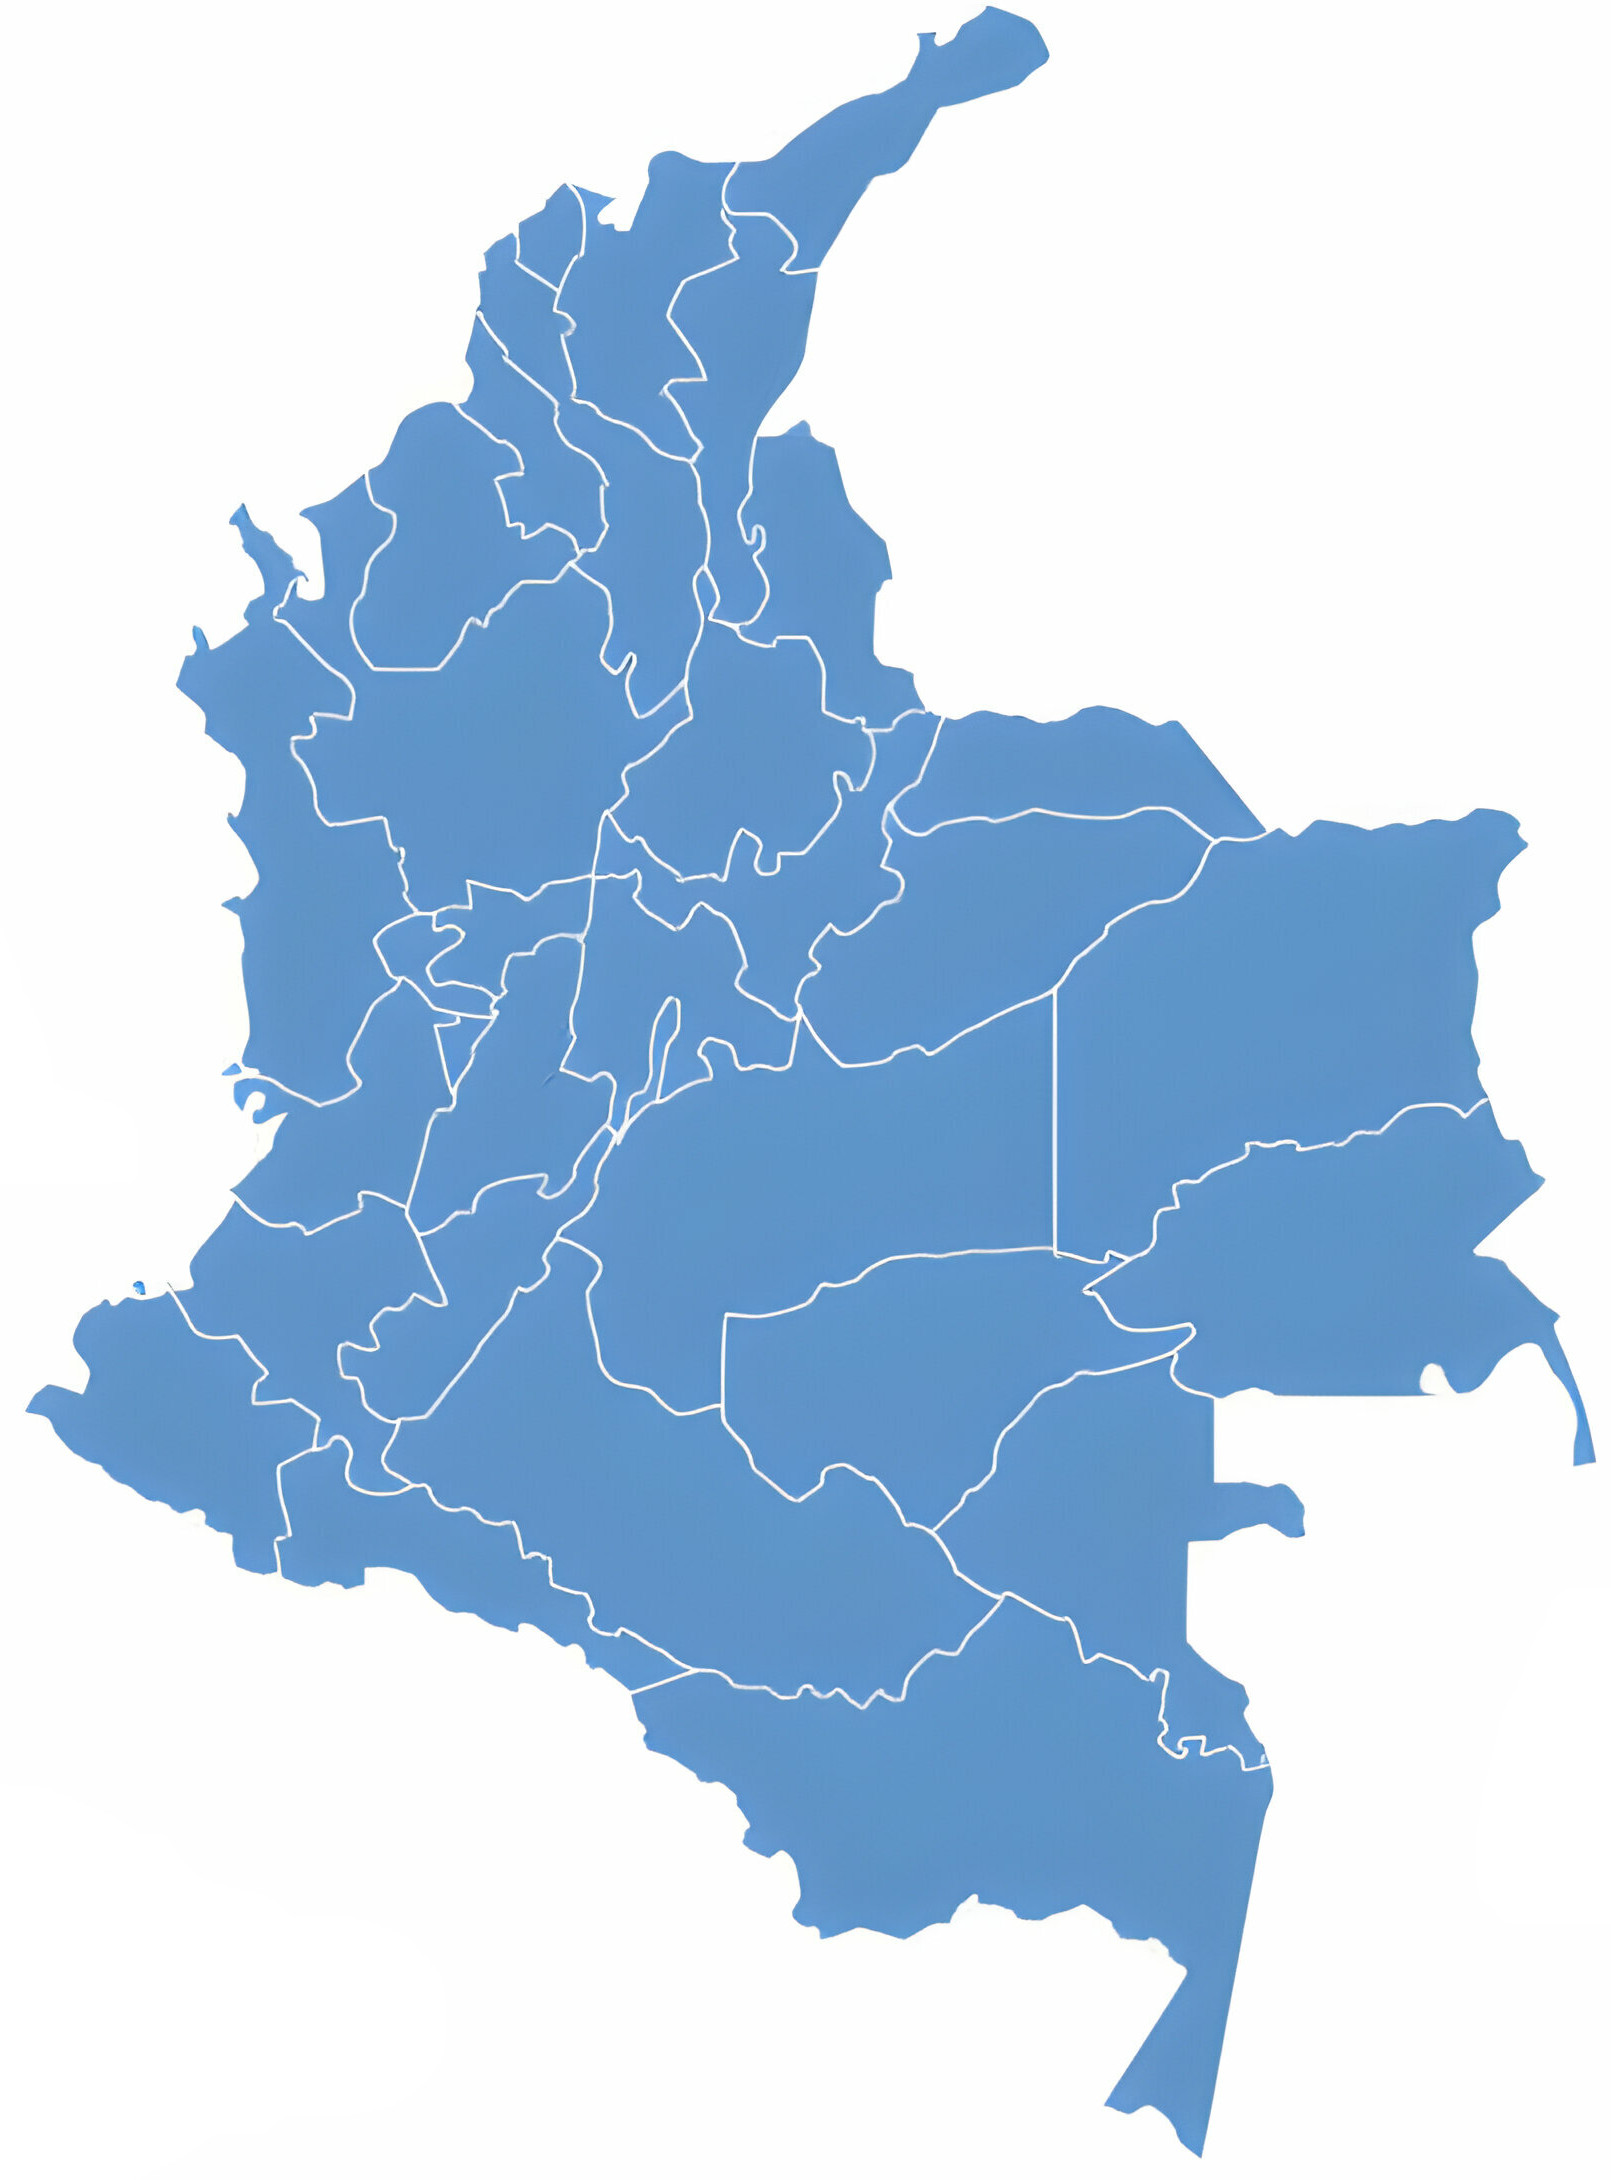
\includegraphics[width=0.5\columnwidth]{images/platanal}
\end{figure}

\end{columns}

\end{frame}
%
\begin{frame}{Motivation}

\framesubtitle{SPRG: Signal Processing and Recognition Group}

Our research group develops \textbf{transdisciplinary data exchange}
since we know that it exposes novel approaches and supports collaborative
discoveries \textbf{across academic areas} \cite{gomezestrategia,aguirre2023feet}.
\begin{columns}[t]

\column[b]{0.5\textwidth}
\begin{itemize}
\item {\scriptsize{}Data heterogeneity.}{\scriptsize\par}
\item {\scriptsize{}Handling unstructured data.}{\scriptsize\par}
\item {\scriptsize{}Real-Time Data Processing and Exchange.}{\scriptsize\par}
\item {\scriptsize{}Privacy and security regulations.}{\scriptsize\par}
\item {\scriptsize{}Interoperability and accessibility.}{\scriptsize\par}
\item {\scriptsize{}Scalability and efficient management.}{\scriptsize\par}
\end{itemize}

\column[b]{0.5\textwidth}

\begin{figure}
\centering{}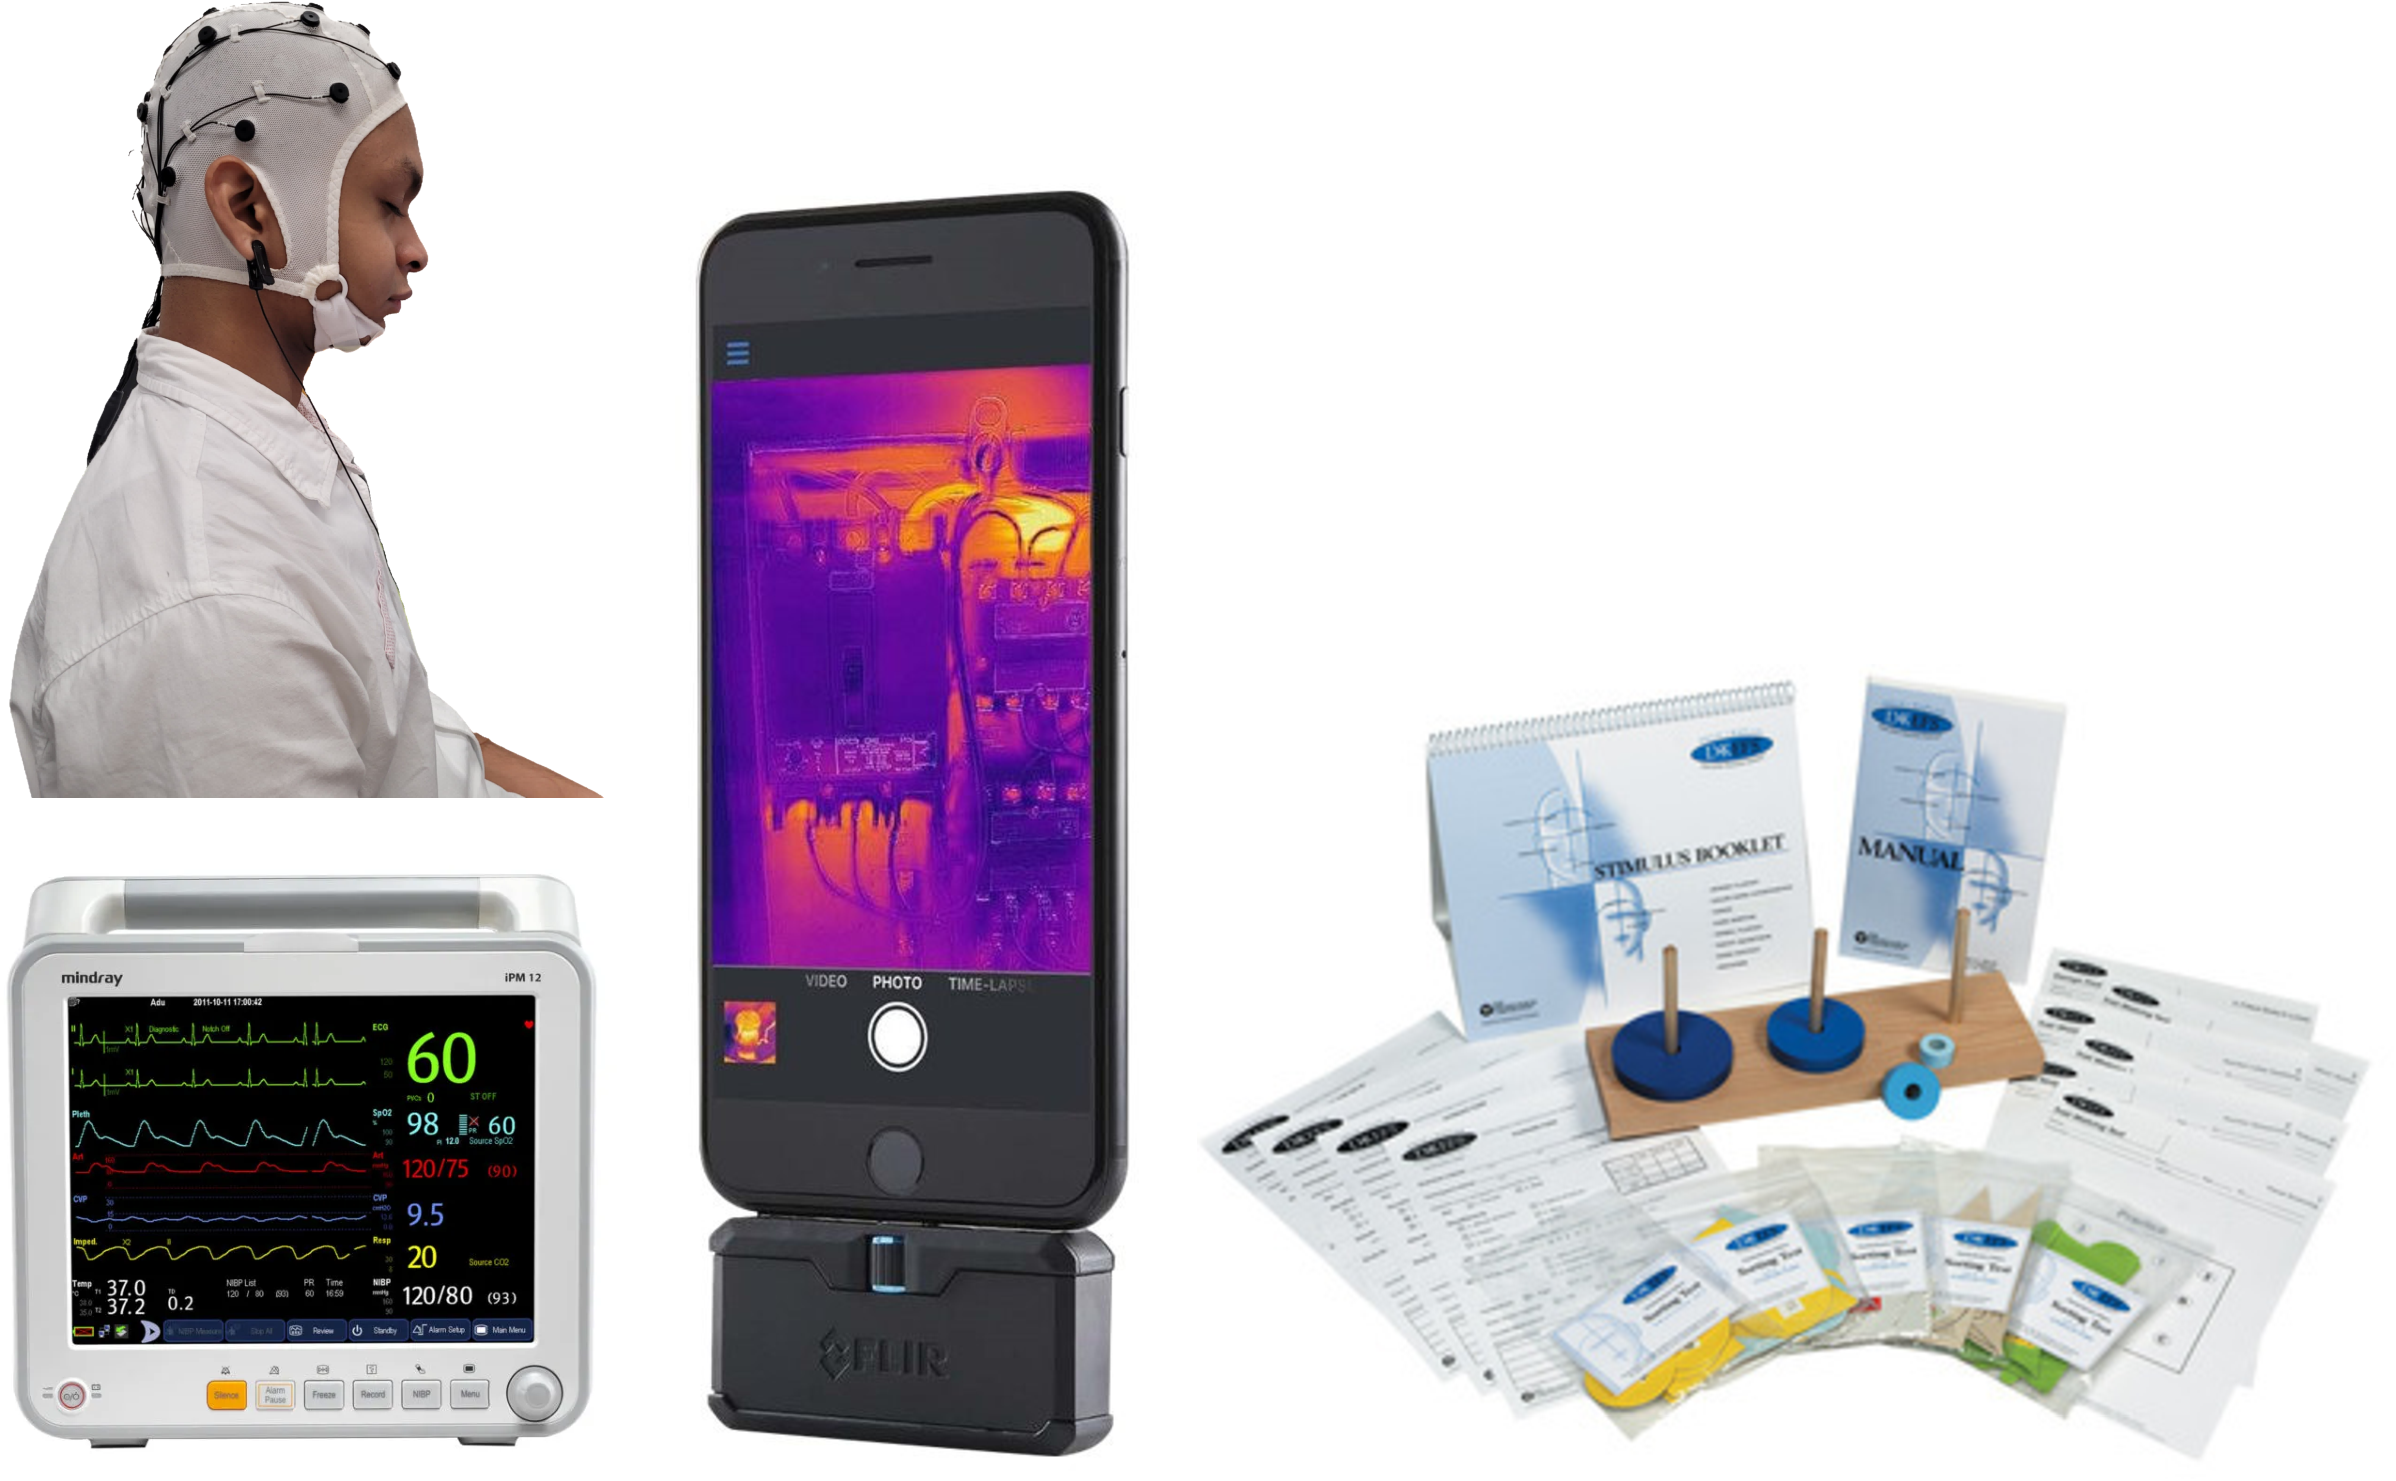
\includegraphics[width=1\columnwidth]{images/research}
\end{figure}

\end{columns}

\end{frame}

\section{Problem statement}
\begin{frame}{Problem statement}

\framesubtitle{Limitations of Data Exchange Methodologies}

 
\begin{columns}[t]

\column{0.5\textwidth}
\begin{description}
\item [{{\scriptsize{}APIs:}}] {\scriptsize{}Request rate, security, and
provider stability/changes limit them \cite{velepucha2023survey}.}{\scriptsize\par}
\end{description}
\vspace{1cm}

\begin{description}
\item [{{\scriptsize{}Messaging:}}] {\scriptsize{}Distributed system scalability,
delivery assurance, state management, and security issues \cite{fang2019integrating}.}{\scriptsize\par}
\end{description}

\column{0.5\textwidth}
\begin{description}
\item [{{\scriptsize{}ETL:}}] {\scriptsize{}Data quality-dependent performance
and complexity concerns with big amounts of different data \cite{abdelhafiz2021sharding}.}{\scriptsize\par}
\end{description}
\vspace{1cm}

\begin{description}
\item [{{\scriptsize{}File\ Transfer:}}] {\scriptsize{}Security, file
size, and bandwidth issues \cite{ordonez2023blockchain,yi2023compound}.}{\scriptsize\par}
\end{description}
\end{columns}

\end{frame}
%
\begin{frame}{Problem statement}

\framesubtitle{API Request Limits}

API request \textbf{rate limits} may cause data transmission difficulties,
especially in multimodal and real-time situations, and make API provider
changes \textbf{harder to adapt} and maintain \cite{Malki2022Impact,Malki2023Combining}.

\begin{figure}
\centering{}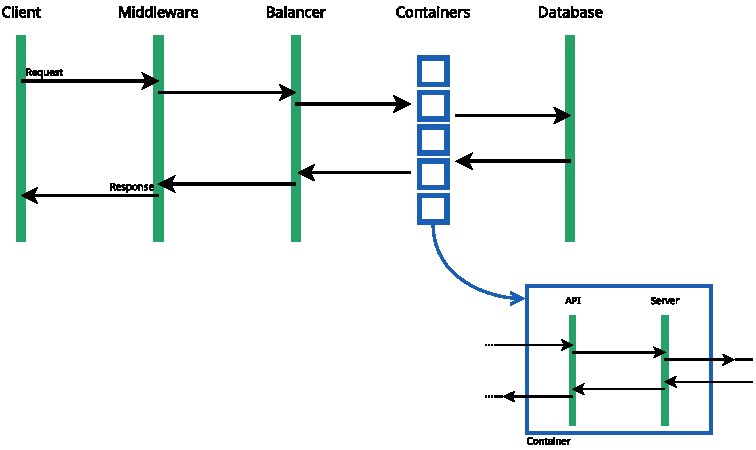
\includegraphics[height=0.35\paperheight]{images/diagrams/API_01}
\end{figure}

\end{frame}
%
\begin{frame}{Problem statement}

\framesubtitle{Messaging Scalability}

Scalability and delivery certainty problems in distributed messaging
systems can lead to the \textbf{loss or delay of messages}, which
can have a severe influence on the \textbf{efficiency and reliability}
of communication in real-time and multimodal contexts \cite{Arellanes2020Evaluating,basin2020scalable}.

\begin{figure}
\centering{}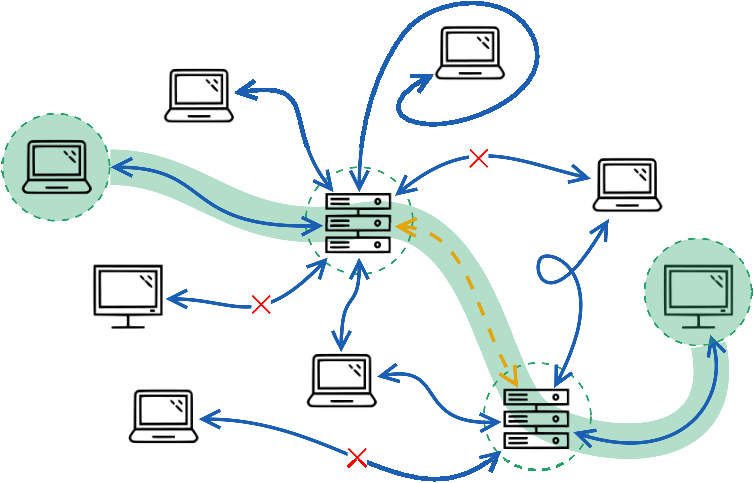
\includegraphics[height=0.35\paperheight]{images/diagrams/MSG_01}
\end{figure}

\end{frame}
%
\begin{frame}{Problem statement}

\framesubtitle{Multimodal ETL \& AI }

Complex multimodal ETL processes can lead to \textbf{inaccurate data
and disruptions} in AI analysis due to challenges with data integration
and real-time data management

\cite{Qaiser2023Comparative,Soussi2021Big-Parallel-ETL:}.

\begin{figure}
\centering{}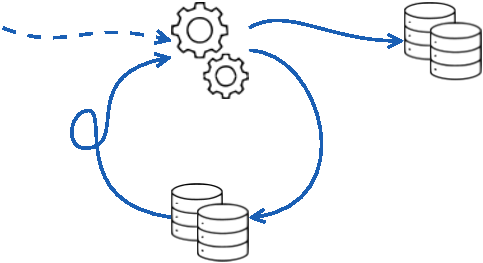
\includegraphics[height=0.35\paperheight]{images/diagrams/ETL_01}
\end{figure}

\end{frame}
%
\begin{frame}{Problem statement}

\framesubtitle{Large-Scale File Transmission}

 

Large-scale file transmission requires efficient and safe administration
of continuous data flow, especially in integrating systems and platforms,
while ensuring data \textbf{integrity} and \textbf{accessibility}
in changing contexts \cite{Zheng2020Design,yin2023network}.

\begin{figure}
\centering{}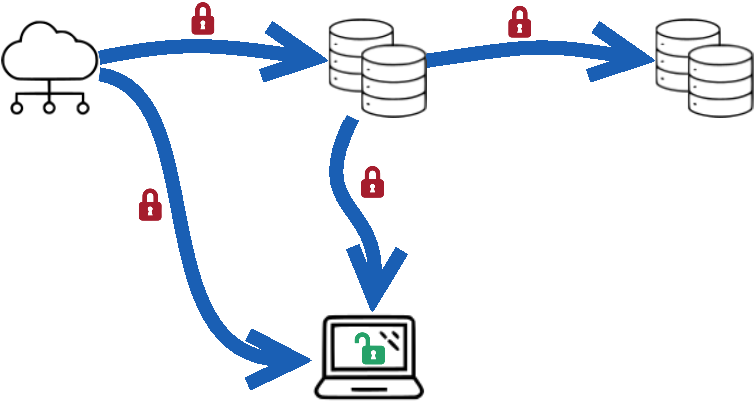
\includegraphics[height=0.35\paperheight]{images/diagrams/FLA_01}
\end{figure}

\end{frame}

\section{State-of-the-Art}
\begin{frame}{State-of-the-Art}

\framesubtitle{APIs: Infrastructure Improving}

\noindent {\footnotesize{}}{\footnotesize\par}

\begin{forest}
  qtree,
  for tree={
    grow=0,             
    parent anchor=children,       
    child anchor=parent, 
    anchor=parent,
    l sep=5mm,  
	font=\tiny,       
  },
  where level=0{
    %grow=0,            
  }{
    if n children=0{folder}{}, 
    edge path'={(!u.parent anchor) -- ++(2.5mm,0) |- (.child anchor)[line width=0.6pt]},
  }
  [Optimization in\\Computer Systems, rotate=90 
    [Resource\\Management, rotate=90
      [Dynamic Resources Management Under Limited Communication Based on Multi-level Agent System \citet{wang2023dynamic}.]
      [Online Task Allocation and Scheduling in Fog IoT using Virtual Bidding \citet{joshi2022online}.]
    ]
    [Communication\\Efficiency, rotate=90 
      [Event-Triggered Communication Network with Limited-Bandwidth Constraint for Multi-Agent Reinforcement Learning \citet{hu2021event}.]
      [Adaptive REST API Testing with Reinforcement Learning \citet{kim2023adaptive}.]
    ]
    [Real-Time\\Systems, rotate=90  
      [On the Design and Implementation of Real-Time Resource Access Protocols \citet{dos2020design}.]
      [Towards Self-Managing Cloud Storage with Reinforcement Learning \citet{noel2019towards}.]
    ]
  ]
\end{forest}

\vfill{}

Limitations in \textbf{real-time API performance} and \textbf{adaptability}
due to static configuration settings.

\end{frame}
%
\begin{frame}{State-of-the-Art}

\framesubtitle{Distributed Messaging: Scalability and Reliability}

\begin{forest}
  qtree,
  for tree={
    grow=0,             
    parent anchor=children,       
    child anchor=parent, 
    anchor=parent,
    l sep=5mm,  
	font=\tiny,       
  },
  where level=0{
    %grow=0,            
  }{
    if n children=0{folder}{}, 
    edge path'={(!u.parent anchor) -- ++(2.5mm,0) |- (.child anchor)[line width=0.6pt]},
  }
  [Distributed Real-Time\\Messaging and Scalability, rotate=90 
    [Event Streaming and\\Async. Communication, rotate=90
      [Reliability enhancements for high-availability systems using distributed event streaming platforms \citet{dincua2023reliability}.]
      [Adaptive Topology for Scalability and Immediacy in Distributed Publish-Subscribe Messaging \citet{banno2020adaptive}.]
    ]
    [IoT and Scalable\\Architectures, rotate=90 
      [Designing a Real-Time IoT Data Streaming Testbed for Horizontally Scalable Analytical Platforms \citet{vstufi2021designing}.]
      [Towards Scalable Cross-Chain Messaging \citet{otavio2023towards}.]
      [PISTIS: An Event-Triggered Real-Time Byzantine-Resilient Protocol Suite \citet{kozhaya2021pistis}.]
    ]
  ]
\end{forest}

\vfill{}
\textbf{Inefficiencies and scalability issues} in distributed messaging
systems affecting real-time communication.
\end{frame}
%
\begin{frame}{State-of-the-Art}

\framesubtitle{AI-Enhanced ETL Processes}

{\footnotesize{}}{\footnotesize\par}

\begin{forest}
  qtree,
  for tree={
    grow=0,             
    parent anchor=children,       
    child anchor=parent, 
    anchor=parent,
    l sep=5mm,  
	font=\tiny,       
  },
  where level=0{
    %grow=0,            
  }{
    if n children=0{folder}{}, 
    edge path'={(!u.parent anchor) -- ++(2.5mm,0) |- (.child anchor)[line width=0.6pt]},
  }
  [Data Integration and\\Real-Time Management, rotate=90 
    [Real-Time Health\\Monitoring, rotate=90
      [Integrating IoT and Machine Learning for Real-Time Patient Health Monitoring with Sensor Networks \citet{vimal2023integrating}.]
      [Data pipeline for real-time energy consumption data management and prediction \citet{im2024data}.]
    ]
    [Advances in Disease\\Detection and Analysis, rotate=90 
      [{Machine Learning Revolution in Early Disease Detection for Healthcare \citet{reddy2023machine}}.]
      [{Deep learning from latent spatiotemporal information of the heart \citet{chang2024deep}}.]
      [Deep Learning Applications in Vessel Dead Reckoning to Deal with Missing Automatic Identification System Data \citet{jmse12010152}.]
    ]
  ]
\end{forest}

\vfill{}

Inefficiencies in processing \textbf{unstructured and temporal data}
in AI-driven multimodal ETL systems.
\end{frame}
%
\begin{frame}{State-of-the-Art}

\framesubtitle{Advancements in Large-Scale File Transmission}

{\footnotesize{}}{\footnotesize\par}

\begin{forest}
  qtree,
  for tree={
    grow=0,             
    parent anchor=children,       
    child anchor=parent, 
    anchor=parent,
    l sep=5mm,  
	font=\tiny,       
  },
  where level=0{
    %grow=0,            
  }{
    if n children=0{folder}{}, 
    edge path'={(!u.parent anchor) -- ++(2.5mm,0) |- (.child anchor)[line width=0.6pt]},
  }
  [Data Flow Management and\\Large-Scale File Transmission, rotate=90 
    [Protocols and\\Network Security, rotate=90
      [{Reliable, Efficient Large-File Delivery over Lossy, Unidirectional Links \citet{van2021reliable}}.]
      [The Design of Intelligent Transportation Video Processing System in Big Data Environment \citet{hao2020design}.]
    ]
    [Coding Techniques and\\Distributed Systems, rotate=90 
      [Design and Optimization of a Distributed File System Based on RDMA \citet{he2023design}.]
      [Network coding for efficient file transfer in narrowband environments \citet{yin2023network}.]
      [Survey of Network Coding Based P2P File Sharing in Large Scale Networks \citet{abudaqa2020survey}.]
    ]
  ]
\end{forest}

\vfill{}
Challenges in ensuring \textbf{efficient and secure} large-scale file
transmission in \textbf{varying network conditions}.
\end{frame}
%
\begin{frame}{Question research}

How can advanced artificial intelligence and machine learning techniques
be used to address important issues in data management and communications
in digital environments? Specifically, how can they improve the flexibility
and effectiveness of real-time APIs, enhance the efficiency and scalability
of distributed messaging systems, process unstructured and temporal
data effectively in multimodal ETL systems, and optimize large-scale
file transmission in different network conditions?
\end{frame}

\section{Aims}
\begin{frame}{General aim}
...

\end{frame}
%
\begin{frame}{Specific aims}

...

\end{frame}

\section{Methodology}
\begin{frame}{Methodology {[}obj1{]}}

Propongo un sistema basado en aprendizaje reforzado que ajuste dinámicamente
los parámetros de configuración de una API REST. Este sistema sería
capaz de modificar en tiempo real aspectos críticos como la configuración
del servidor (que opera en un entorno basado en contenedores) y la
interacción con la base de datos. La idea central es que el sistema
aprenda y se adapte automáticamente a las variaciones en el uso y
demanda de la API, optimizando recursos, mejorando el rendimiento
y garantizando una gestión eficiente de la tasa de solicitudes. Este
enfoque busca combinar la flexibilidad y escalabilidad de los contenedores
con la inteligencia y adaptabilidad proporcionadas por el aprendizaje
reforzado, enfocándose en mantener un alto nivel de servicio y disponibilidad
de la API, incluso ante cambios dinámicos en el entorno y la demanda.

El problema a abordar es cómo superar las limitaciones de tasa de
solicitudes de API, que generan dificultades en la transmisión de
datos en escenarios multimodales y en tiempo real, y complican la
adaptación y mantenimiento cuando se cambian los proveedores de API.

\end{frame}
%
\begin{frame}{Methodology {[}obj2{]}}

Propongo un sistema avanzado de mensajería distribuida, basado en
una red de malla donde cada nodo puede enviar y recibir mensajes.
Esta red integra específicamente tecnologías de inteligencia artificial
para optimizar su funcionamiento: utiliza Redes Neuronales Recurrentes
(RNN) para el enrutamiento dinámico y predecir la congestión de la
red, técnicas de clustering para el balanceo equitativo de carga,
Autoencoders para la detección de anomalías y seguridad, y aprendizaje
por refuerzo para la optimización constante de rutas. Además, emplea
modelos de regresión para predecir fallos de nodos y algoritmos de
segmentación de usuarios para personalizar la experiencia de comunicación.
Este enfoque brinda una red más eficiente, segura y adaptable, mejorando
la entrega de mensajes y la experiencia del usuario, al mismo tiempo
que aumenta la resistencia de la red a fallos y ataques.
\end{frame}
%
\begin{frame}{Methodology {[}obj3{]}}

Propongo un sistema orientado a optimizar los procesos de ETL multimodal
en entornos de inteligencia artificial a través de algoritmos avanzados
de aprendizaje automático y aprendizaje profundo, centrado en la integración
eficiente y procesamiento de datos no estructurados mediante redes
neuronales convolucionales y la gestión dinámica de secuencias de
datos temporales utilizando redes neuronales recurrentes. Este enfoque
práctico involucra el desarrollo de prototipos y su validación en
escenarios de uso real, destacando aplicaciones como la monitorización
en tiempo real y el análisis de grandes conjuntos de datos, con el
objetivo de mejorar significativamente la precisión, eficiencia y
capacidad de respuesta de los sistemas de ETL, proporcionando un marco
concreto y aplicable para enfrentar desafíos actuales en el procesamiento
de datos en IA.
\end{frame}
%
\begin{frame}{Methodology {[}obj4{]}}

Para optimizar la transmisión de archivos a gran escala, propongo
un sistema de servidor inteligente capaz de adaptarse en tiempo real
a las condiciones de conexión y restricciones del cliente, como la
pérdida de paquetes y variaciones en el ancho de banda. Este sistema
utilizará Redes Neuronales Recurrentes, en particular Long Short-Term
Memory (LSTM), para monitorear y predecir de manera continua y precisa
las condiciones de la red del cliente. Basándose en esta información,
el servidor ajustará dinámicamente la tasa de transmisión de archivos,
seleccionará protocolos de comunicación óptimos y aplicará técnicas
de compresión de datos para adaptarse a las limitaciones del cliente.
Además, el sistema contará con mecanismos de aprendizaje continuo
que le permitirán mejorar progresivamente su capacidad de adaptación,
asegurando una transmisión eficiente y confiable en un amplio rango
de condiciones de red. Esta propuesta busca proporcionar una experiencia
de usuario óptima con un enfoque proactivo y adaptable a las necesidades
específicas de cada cliente.
\end{frame}

\section{Academic advances}
\begin{frame}{Academic advances}

\framesubtitle{Papers, patents and software registers}
\begin{itemize}
\item {[}2023{]} Paper published...
\item {[}2022{]} The systems were submitted to the \textbf{Crearlo no es
suficiente} summons for a \emph{patentability search process} with
the \emph{Universidad Nacional de Colombia sede Manizales} as main
beneficiary with the title \textbf{\textquotedbl MÉTODO Y SISTEMA
PARA LA SINCRONIZACIÓN DE MARCADORES ASOCIADOS A SISTEMAS DE INTERFAZ
CEREBRO-COMPUTADOR\textquotedbl}, postulation \emph{ID 343 }and
Application number \emph{NC2022/0007405} from May 28, 2022.
\item {[}2022{]} A script developed with BCI-Framework for\textbf{ Motor
imagery paradigm with game-based stimulus (Pacman interface)} was
submitted to the software register in the \emph{Universidad Nacional
de Colombia sede Manizales}.
\end{itemize}
\end{frame}

\section{Acknowledgements}
\begin{frame}{Acknowledgements}

...
\end{frame}

\section{References}
\begin{frame}[allowframebreaks]{References}

{\tiny{}\bibliographystyle{apalike}
\bibliography{references}
}{\tiny\par}

\end{frame}

\end{document}
